\section{Design}

\subsection{Dashboard design}
A very important aspect the group has had to concider, is which design pattern
to model the dashboard after. A design pattern is a form of template, which in
this case, dictates how the different classes communicate. A relevant design
pattern is the MVC (Model - View - Controller). This pattern separates the
database (data-related logic), the GUI (UI logic) and the logic (interface
between the two) into different layers, and thereby helps keep separation of
concerns. The controller manages input from the user, and forwards it to either
the model, to retrieve or store data, or the view, to present data to the user.

The group has decided to use the MVC design pattern, thus making it possible to
work on the different elements of the system (GUI, database, logic) separately.
To ensure that these different parts of the system can communicate, a
'contract', in this case the controller, should be created.

A visualisation of the MVC pattern can be seen in figure \ref{figure:MVC_model}

\begin{figure}[ht]
    \centering
    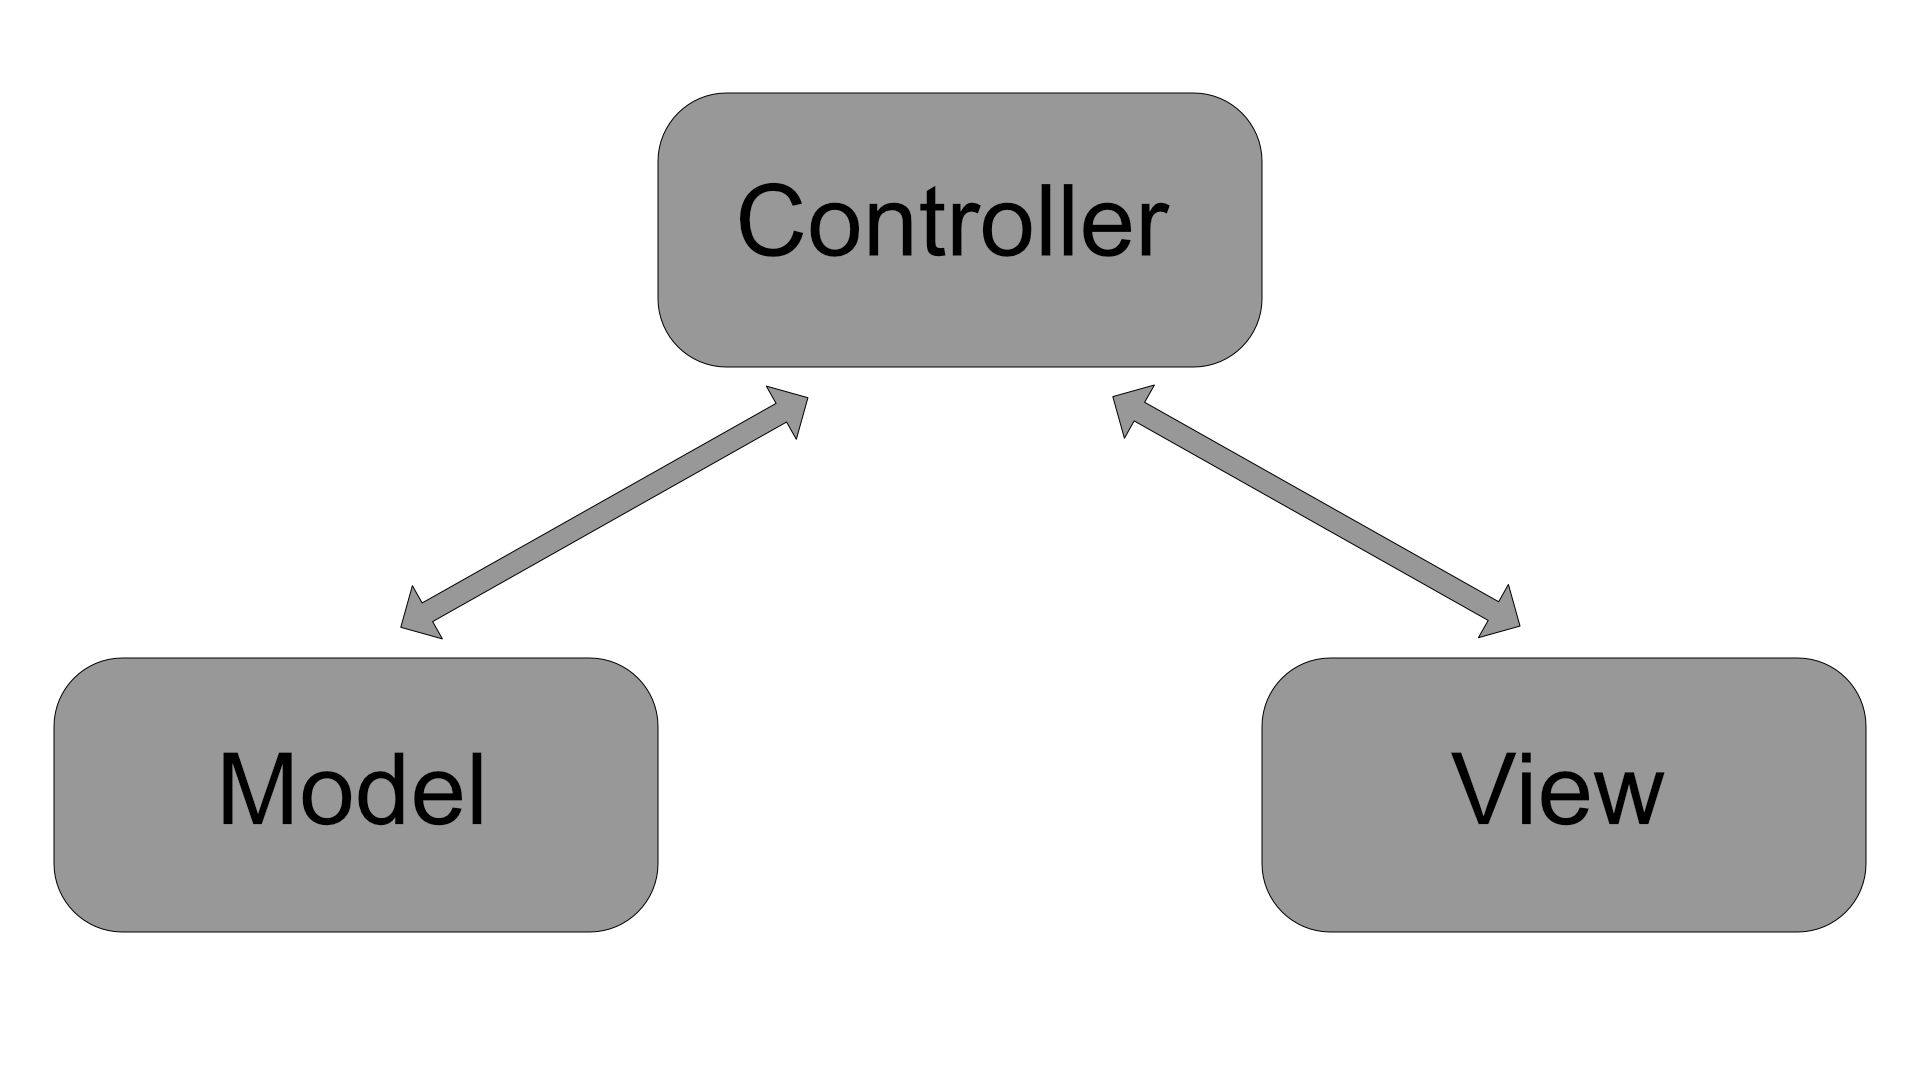
\includegraphics[scale=0.35]{images/MVC_model.jpg}
    \caption{MVC model}
    \label{figure:MVC_model}
\end{figure}